\documentclass[a4paper, 11pt]{article}
\usepackage{comment} 
\usepackage{fullpage}
\usepackage{hyperref}
\usepackage{amsmath}
\usepackage{environ}
\usepackage{tabto,enumitem}
\usepackage{lipsum}
\usepackage{float}
\usepackage{tabto}
\usepackage{booktabs} 
\usepackage{graphicx}
\usepackage{graphics}
\usepackage{gensymb}

\usepackage[ruled]{algorithm2e}
\renewcommand{\algorithmcfname}{ALGORITHM}

\title{ETERNITY: FUNCTIONS}								
\author{Apekshaba Gohil}						
\date{}

\makeatletter
\let\thetitle\@title
\let\theauthor\@author
\let\thedate\@date
\makeatother

\begin{document}

\begin{titlepage}
	\centering
    \vspace*{0.5 cm}
\begin{center}    \textsc{\Large Concordia University}\\[2.0 cm]	\end{center}
	\textsc{\Large  SOEN 6011 - Software Engineering Process }\\[0.5 cm]
	\rule{\linewidth}{0.2 mm} \\[0.4 cm]
	{ \huge \textbf \thetitle}\\[0.2 cm]
	{ \huge \textbf{tax(x)}}
	\rule{\linewidth}{0.2 mm} \\[1.5 cm]

\begin{center}   {\Large Deliverable final}\\[2.0 cm]
\end{center}	
\begin{center}   {\Large \textbf{\theauthor}} \\[0.2 cm]
                 {\large Student ID : 40203058 }\\[1.5 cm]
              
                 {\large https://github.com/Apekshaba/SOEN-6011}
\end{center}
	
\end{titlepage}

\section*{Problem 1}
\section{Introduction}

F2:  $f(x)= tan(x)$ is a trigonometric tangent function where x is an angle at which the tangent is found. Here, x is an angle in rad. This function is one of the most commonly used function in mathematics.

\section{Domain \& Co-Domain}

\subsection{Domain}
\begin{itemize}
  \item it includes all the real numbers,
   but not the values for x where cos(x) is zero, because tan can also be written as the ratio of sine and cosine functions. So the domain will contain all the real numbers excluding  $ {( 2n+1)}\frac{\pi}{2} $	
 \end{itemize}
  
 \subsection{Co-Domain}
 \begin{itemize}
  \item  For the negative value of an angle ,the tangent will also be negative. 
  \item  For the positive values of an angle, the tangent will also be positive.
\end{itemize}

 \subsection{Range}
 \begin{itemize}
     \item The range of the tan function is R where, R is a set of all real numbers.
 \end{itemize}
    
 \subsection{Restrictions} 
 \begin{itemize}
  \item  for the angle value of 90\degree  tan is not defined.  
\end{itemize}

\section{Characteristics}

\begin{itemize}
  \item $\boldsymbol{Growth}$ :When the value of angle lies between every alternate section of $\frac{\pi}{2}$ the tangent function seems to be increasing until it reaches the multiple of $90\degree$, where it's not defined.

  \item $\boldsymbol{Decay}$ : When the value of angle starting from $\frac{\pi}{2}$ to the next subsection of $\frac{\pi}{2}$, tangent function seems to be decreasing until it reaches the undefined state. as shown in the $Figure^{[1]}$.
  
  \item $ \textbf{Injectivity \& Surjectivity}$ : The tangent function is both injective and surjective and so it is  called bijective function.
  
  \begin{figure}[H]
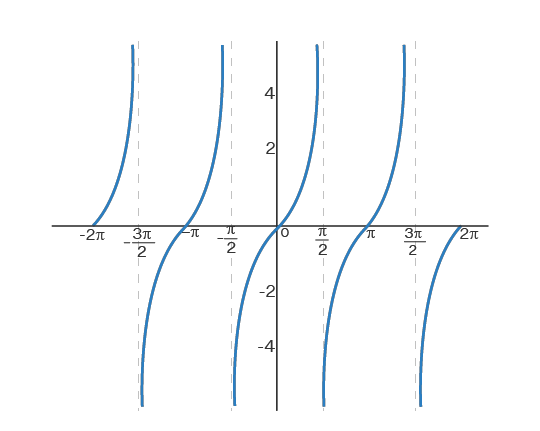
\includegraphics[width=18cm]{TanxGraph.png }
\caption{curve growth and Decay graph of tangent function.}
\label{exp}
\end{figure}
\end{itemize}

\newpage
\section*{Problem 2}
\section*{Requirements}
    \subsection*{First Requirement}
    \begin{itemize}
        \item \textbf{ID = } FR1
        \item \textbf{Type = } Functional Requirements
        \item \textbf{Version = } 1.0
        \item \textbf{Difficulty = } Easy
        \item \textbf{Description = }System shall take an input X which is nothing but the angle for which the tangent is to be found, ahich then is converted into radians and the output which is a tangent value for that value of angle is given. \\
        Example :for  $x = 45, tan(x) = 0.99924342$
    \end{itemize}
    \subsection*{Second Requirement}
    \begin{itemize}
        \item \textbf{ID = } FR2
        \item \textbf{Type = } Functional Requirements
        \item \textbf{Version = } 1.0
        \item \textbf{Difficulty = } Easy
        \item \textbf{Description = } $tan(x)$ is dependent on the $sin(x) and cos(x)$ functions which are expanded using Taylor series expansion.\\
    \end{itemize}
    \subsection*{Third Requirement}
    \begin{itemize}
        \item \textbf{ID = } FR3
        \item \textbf{Type = } Functional Requirements
        \item \textbf{Version = } 1.0
        \item \textbf{Difficulty = } Easy
        \item \textbf{Description = }  User shall give an input from all real numbers for x but the values for which cos(X) is zero.  
    \end{itemize}
    \subsection*{Fourth  Requirement}
    \begin{itemize}
        \item \textbf{ID = } FR4
        \item \textbf{Type = } Functional Requirements
        \item \textbf{Version = } 1.0
        \item \textbf{Difficulty = } Easy
        \item \textbf{Description = }when user gives other input then integer that is string then system shall not accept and will ask to provide proper response after checking it using the Util function inValidRange.
    \end{itemize}
        \subsection*{Fifth  Requirement}
    \begin{itemize}
        \item \textbf{ID = } FR5
        \item \textbf{Type = } Functional Requirements
        \item \textbf{Version = } 1.0
        \item \textbf{Difficulty = } Easy
        \item \textbf{Description = }when user provides a value that is out of range for the Double variable's valid range, It says value out of range.
    \end{itemize}

\newpage
\section*{Problem 3}
\section*{Pseudocode and Algorithm}
Calculate: $f(x) = tan(x)$ \\[0.5 cm]
Consider $tan(x) = \frac{sin(x)}{cos(x)}$
\begin{algorithm}
\caption{Iterative algorithm to calculate $tan(x)$ using Taylor series expansion}\\

\begin{algorithmic} 
1. function \textbf{sin(x)}\\
\textbf{in: } double radian\\
\textbf{out: } double sinX\\
2. \STATE $pow \leftarrow 1$\\
3. \STATE $sinX \leftarrow 0.0$\\
4. for {$Iterator \leq 15$} do\\
5.\qquad \STATE $current\_term \leftarrow 0.0$\\
6. \qquad \STATE if {$Iterator\mod 2 \ == 0$}\\
7. \qquad \STATE $current\_term  \leftarrow -tan.power(radians, pow)$\\
8. \qquad \STATE else\\
9. \qquad \STATE $current\_term  \leftarrow tan.power(radians, pow)$\\
10.\qquad \STATE $sinX \leftarrow sinX+current\_term$\\
11.\qquad \STATE $pow \leftarrow pow+2$\\
12. end for\\
13. \STATE return sinX \\
14. function \textbf{cos(x)}\\
\textbf{in: } double radian\\
\textbf{out: } double cosX\\
15. \STATE $pow \leftarrow 0$\\
16. \STATE $cosX \leftarrow 0.0$\\
17. for {$Iterator \leq 15$} do\\
18.\qquad \STATE $current\_term \leftarrow 0.0$\\
19. \qquad \STATE if {$Iterator\mod 2 \ == 0$}\\
20. \qquad \STATE $current\_term  \leftarrow tan.power(radians, pow)$\\
21. \qquad \STATE else\\
22. \qquad \STATE $current\_term  \leftarrow -tan.power(radians, pow)$\\
23. \qquad \STATE $cosX \leftarrow cosX+current\_term$\\
24. \qquad \STATE $pow \leftarrow pow+2$\\
25. end for\\
26. \STATE return cosX \\
27. function \textbf{getFact(power)}\\
\textbf{in: } Integer power\\
\textbf{out: } Integer fact\\
28. \STATE $fact \leftarrow 1$\\
29. for {$Iterator \leq power$} do\\
30. \qquad \STATE $fact \leftarrow fact*Iterator$\\
31. end for\\
32. \STATE return fact\\
33. function \textbf{power(radian, exponent)}\\
\textbf{in: } double radian, exponent\\
\textbf{out: } double res\\
34. \STATE $res = 1$\\
35. while  \STATE $exponent != 0$  do\\
36. \qquad $res = res*radian$ \\
37. \qquad $--exponent$ \\
38. end while \\
39. \STATE return res\\ 
\end{algorithmic}
\end{algorithm}

\newpage
Here, I keep track of our result in a variables called sinX and cosX in two different functions, which are initially set to be equal to 0.0. after that we are simply calling a power function for the angle x which keeps track of the results into $current\_term$ which was then appended to the final results be them sinX and cosX and returned at the time of a call from tan(X) function call\\

\begin{algorithm}
\caption{Recursive algorithms in order to receive the results of tanx using exponential functions}\\
\begin{algorithmic}
1.\Procedure{epowerx}{$x$}\\
2.\For{$i\gets0$  to $maxdepth$ }\\ 
3.\State $result = 1 + x * result / i$\\
4.  endFor\\
5.  endProcedure\\
6.\State $epowerX = epowerx(x)$\\
7.\State $epowernegativeX = epowerx(-x)$\\
8.\State $tanX= (epowerX - epowernegativeX) / iterator(epowerX + epowernegativeX)$\\
\end{algorithmic}

\end{algorithm} 
Here, there's a common exponential function has been defined which returns the positive and negetive exponential power of constant e of x times,
The result of tanX is finally stored using the function and exponential function based on the formula of $tan(x) = \frac{(e^{ix}-e^{-ix})}{i(e^{ix}+e^{-ix})}$

\newpage


\subsection*{Advantages and Disadvantages}
\subsubsection*{Algorithm 1:}
Advantages:\\
1. In terms of space complexity, iterative algorithms don't suffer from stack overflow because all operations are done on the heap. and later alocated the space to store the final result \\
2. Easy to read and follow since the format is easy to understand.\\
Disadvantages:\\
1. The time complexity of the iterative algorithm is $O (n)$, hence it is not very efficient for larger inputs in terms of time.  \\
2. Proper terminating condition for loop is needed or else we might get stuck in infinite loop.
\subsubsection*{Algorithm 2:}
Advantages: \\ 
1. The time complexity of our recursive algorithm is $O (log n)$. Our version of recursive algorithm is optimized and tail recursive so that we don't get stack overflow error. here the implementation and soc is lesser and easier compare to iterative algorithm. \\
2. Recursion has higher maintainability than loop. There's little to no modification needed if we handle base case correctly\\
Disadvantages:\\
1. When using recursion, system continuously allocates memory space, which leads to the stack overflow issue. \\
2. The algorithm is highly crucial at the time of handling base cases and might misbehave at the time of edge cases. 
3. It is not really very readable since most of the part is in binary mathematical format.
\subsubsection*{Conclusion}
My decision of going with the Iterative algorithm using Taylor series was mostly because of code re-usability simple and modular design, even though it might take a little extra time than a recursive algorithm using Exponential function would take having the computer space managed quite well it has been proven the best decision.

\newpage
\section*{Problem 4}
\subsection{Debugger}
In the project, I have used the Intellij IDE debugger to debug the code. The
Intellij IDE provides many debugging tools and views grouped in debug
perspective to debug effectively and efficiently. this debugger provides
functions to run the code step by step and track the values of variables while
debugging. 
\subsection*{Advantages and Disadvantages}
Advantages: \\[0.2 cm]
• The values of variables can be changed at debugging mode on the fly.\\
• It has step filtering functions to step into or step over a statement\\
• It offers a feature to show the logical structure that allows viewing the
object in another meaningful structure/view.\\
• It offers event based breakpoints.\\[0.2 cm]
Disadvantages:\\[0.2 cm]
• Debugging real time/multi-thread programs becomes harder as it involves huge lines of code and it’s better to perform testing using test
cases.\\
\subsection{Quality Attributes:}
\subsubsection{ correctness:}
The program is tested for all the possible values of an angle Tangent function can return.
\subsubsection{space-efficient:}
The function implemented is space-effiecient since all the variables are tacked into heap and stored into memory at the time of passing it.
\subsubsection{portable and maintainable:}
The program is devided into three classes which make it effective and easy to understand and maintain, that is breakout into one class will be easier to handle without making any possible damage to the other files.
\subsubsection{Robust:}
The program is tested for all faulty inputs and outputs, and all possible outliers to check it's robustness.
\subsubsection{Usable:}
The program is made useable so that anyone can easily understand and make changes according to their requirements.
\subsubsection{ time-efficient:}
The program is made to be less time consuming by efficiently using the loops to not interrupt abruptly.


\begin{figure}[H]
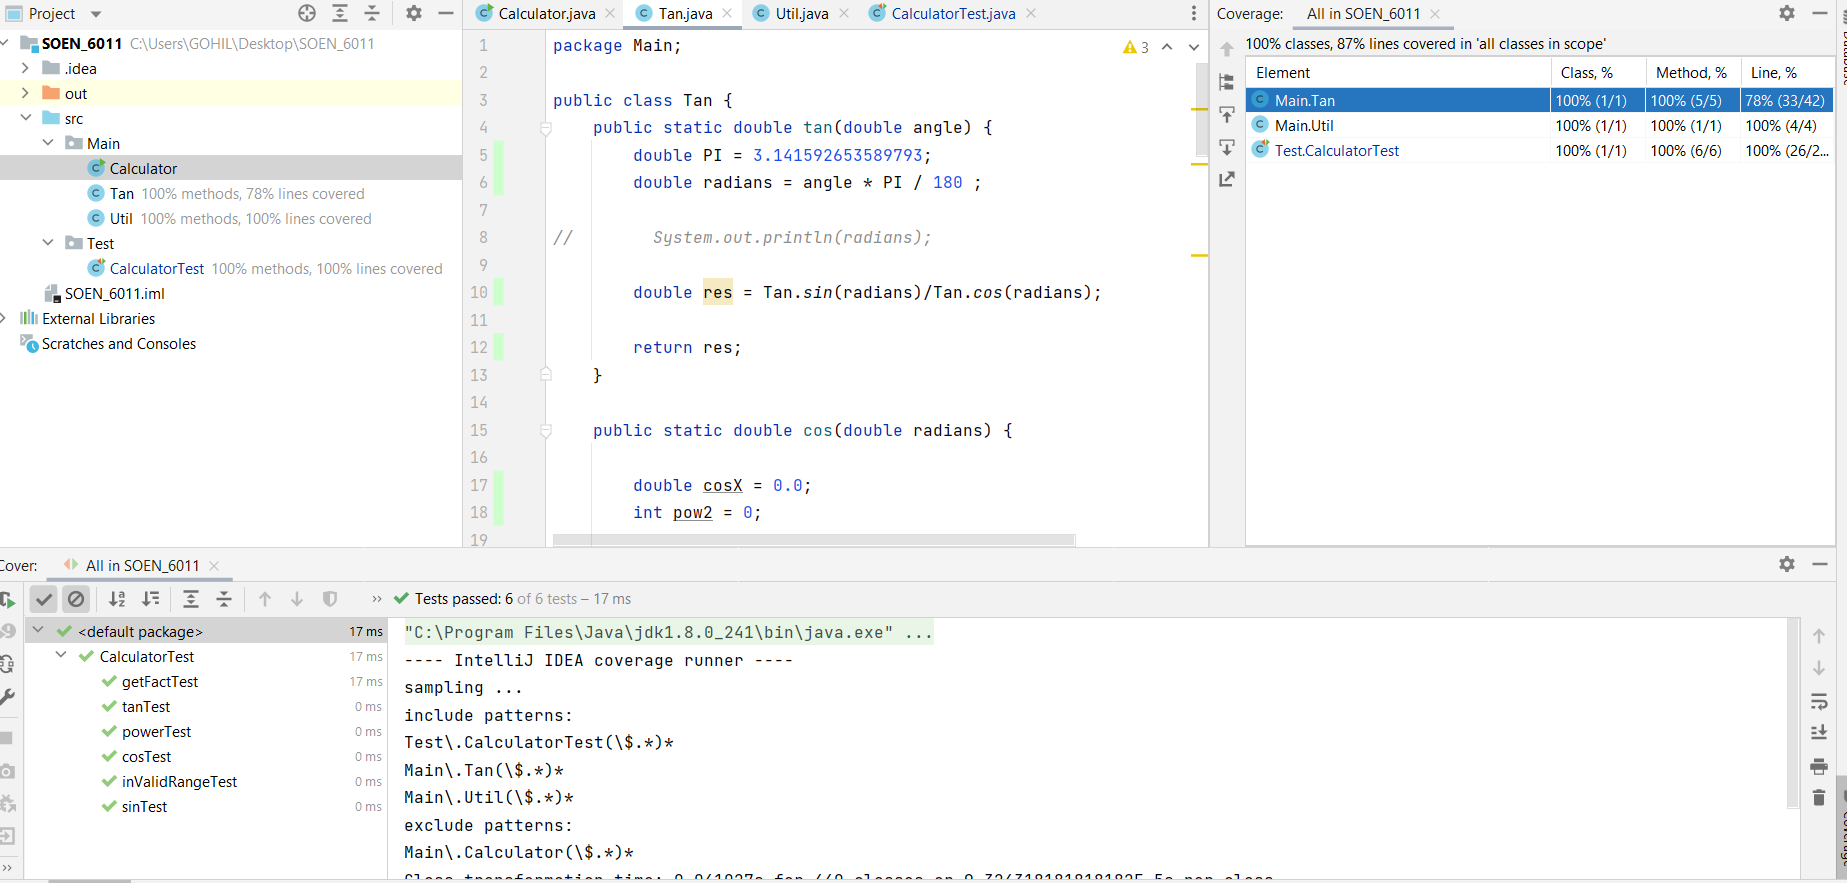
\includegraphics[width=18cm]{debugger1.png}
\caption{The snapshot of the debugger which has included the coverage of the functions and the display of the successful tests has been shown .}
\label{exp}
\end{figure}

\begin{figure}[H]
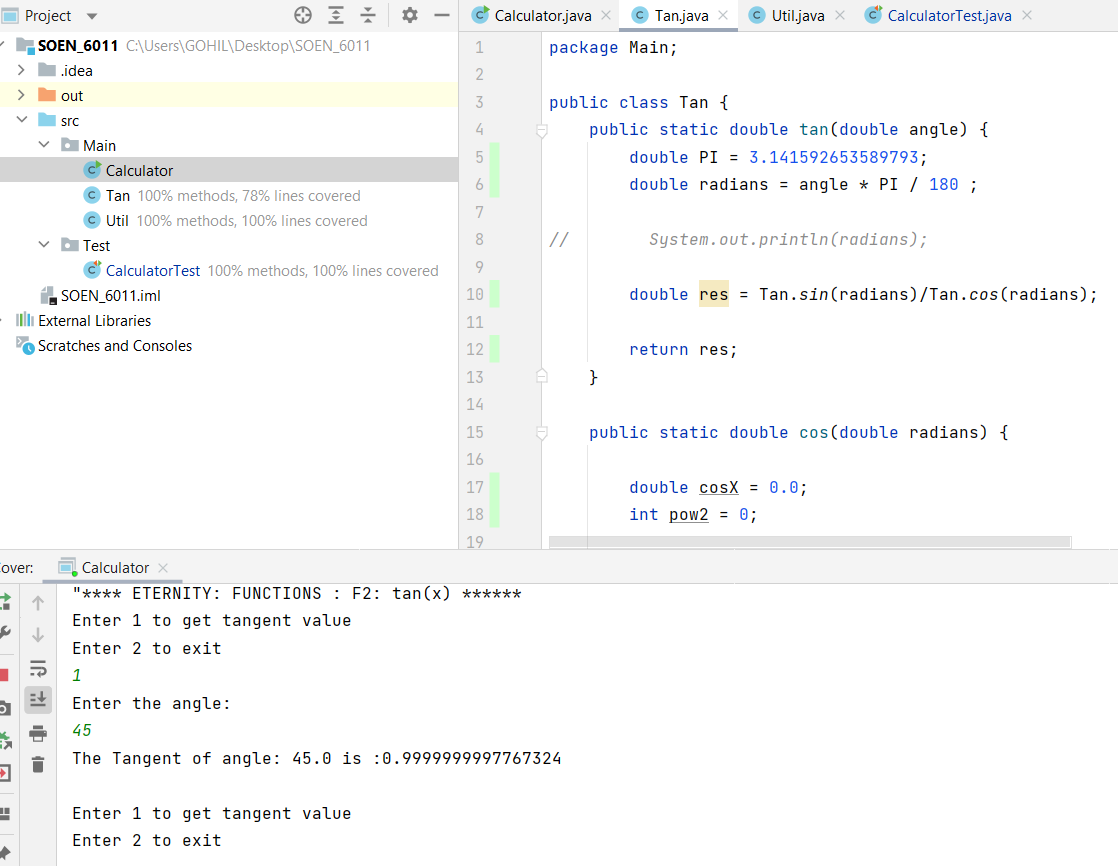
\includegraphics[width=18cm]{debugger2.png}
\caption{The snapshot of the debugger which has a case where it ran perfectly for the value in range}
\label{exp}
\end{figure}

\begin{figure}[H]
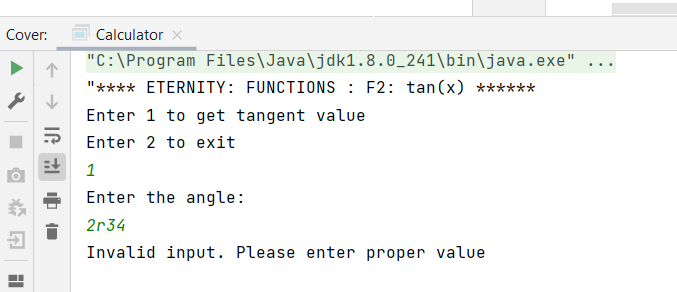
\includegraphics[width=18cm]{debugger3.png}
\caption{The snapshot of the debugger where the error and exceptions has been handled. }
\label{exp}
\end{figure}

\newpage
\begin{thebibliography}{9}
\bibitem{MathBitsNotebook}
MathBitsNotebook,\\
\url{https://mathbitsnotebook.com/Algebra1/FunctionGraphs/FNGTypeExponential.html}
\bibitem{TutorialsPoint}
TutorialsPoint,\\
\url{https://www.tutorialspoint.com/java/lang/math_pow.htm}
\bibitem{R. T. Barker and D. W. Biers} R. T. Barker and D. W. Biers,   "Software usability testing: Do user self-consciousness and the laboratory environment make any difference?" in Part 2 (of 2), October 24, 1994 - October 28, 1994, .
\bibitem{S. L. Sparagen and A. Riback}  S. L. Sparagen and A. Riback, "Flexible software interface design," Ergonomics Des., vol. 7, (4), pp. 4-8, 1999.
\bibitem{M. Hon, G. Russell and M. Welch} M. Hon, G. Russell and M. Welch, "Open source software considerations for law enforcement," IT Professional, vol. 12, (6), pp. 18-23, 2010. Available: http://dx.doi.org/10.1109/MITP.2010.121. DOI: 10.1109/MITP.2010.121.
\bibitem{J. Ragot, D. Maquin and A. Kondo} J. Ragot, D. Maquin and A. Kondo, "Control design for loop transfer recovery," in Part 1 (of 3), October 2, 1994 - October 5, 1994, .
\bibitem{B. Haberman and H. Averbuch} B. Haberman and H. Averbuch, "The case of base cases: Why are they so difficult to recognize? student difficulties with recursion," in ITiCSE 2002 - Proceedings of the 7th Annual SIGCSE Conference on Innovation and Technology in Computer Science Education, June 24, 2002 - June 28, 2002, Available: http://dx.doi.org/10.1145/544414.544441. DOI: 10.1145/544414.544441.
\end{thebibliography}

\end{document}